In order to test the proposed A* algorithm, an electric power system (EPS) model based a Florida feeder available in the SUNGRIN report \cite{SUNGRIN} was collected. Fig. \ref{fig:simulation_grid} shows a one-line diagram of the whole system used for testing the algorithm. The dashed borders mark the section of the feeder modified to create a microgrid similar to the one shown in Fig. \ref{fig:system_arch}. The PV and load inside the microgrid are modeled using the load and solar data collected from the SUNGRIN project. An energy storage (ES) system is included to construct the microgrid. Table \ref{tab:solar_pv} shows the physical parameters of the PV plant and its inverter. The energy storage (ES) used in the modeled microgrid has the parameters shown in table \ref{tab:es}. The levelized cost of energy (LCOE)  of the energy storage system $R_{ESS}$ is calculated using (\ref{eq:R_ESS}).

\begin{figure}[!ht]
    \centering
    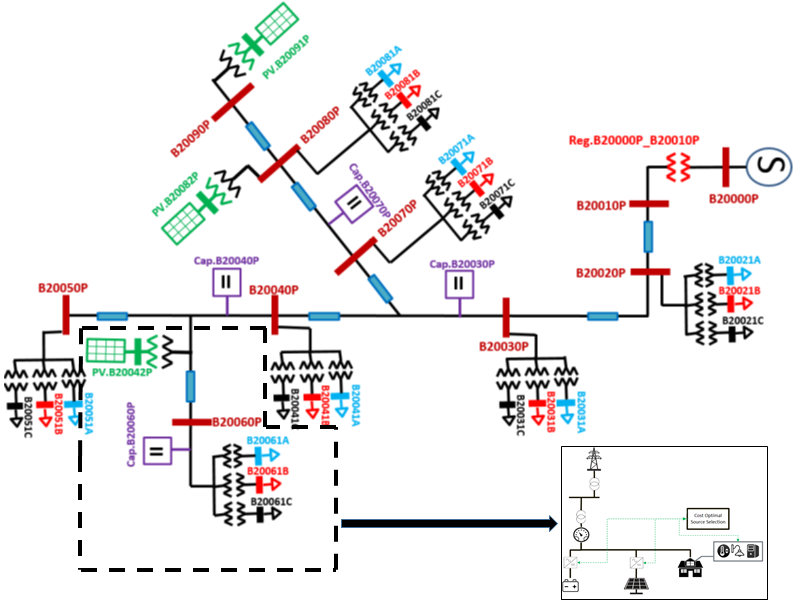
\includegraphics[width = 0.8\linewidth]{figs/A8/simulation_grid.png}
    \caption{Simulated system}
    \label{fig:simulation_grid}
\end{figure}


\begin{equation}
\label{eq:R_ESS}
R_{ESS} = \dfrac{ES_{tot}}{Cyc\cdot ES_{Cap}\cdot DoD\cdot \eta_{r}},
\end{equation}

Where $ES_{tot}$ is the total cost of the ES system, $DoD$ is the desired depth-of-discharge of the ES system, $Cyc$ is the total number of cycles under warranty at depth-of-discharge, $ES_{Cap}$ is the total energy capacity of the ES system, and $\eta_r$ is the round-trip efficiency of the system. The data used to calculate the $R_{ESS}$ price used in the study were obtained from publicly available data on a commercial ES solution \cite{tesla_powerpack_2018}. 

%%%%%%%%PV%%%%%%%%%%%%%%%%%%%%%%%%%%%%%%%%%%%
\begin{table}[!ht]
%\normalsize
%\renewcommand{\arraystretch}{1}
\caption{PV System Specifications}
\label{tab:solar_pv}
\centering
    \begin{tabular}{ | l | p{3cm} | }
    \hline
    \textbf{PV System Parameters} & \textbf{Value} \\ \hline
    PV Panels Rating (\(P_{PV}\)) & 875 kW  \\ \hline
    Inverter Rating (\(S_{PV}\)) & 900 kVA \\ \hline
    Power Factor Range (\(pf_{PV}\)) & 0.8-1.0  \\ \hline
    Max. Reactive Power (\(\overline{Q_{PV}}\)) & 540 kVAR \\ \hline
    Min. Reactive Power (\(\underline{Q_{PV}}\)) & -540 kVAR \\ \hline
    LCOE (\(r_{PV}\)) & 2.51 c/kWh \\ \hline
    \end{tabular}
    \begin{tabular}{l}
    \end{tabular}
\end{table}
%%%%%%%%PV%%%%%%%%%%%%%%%%%%%%%%%%%%%%%%%%%%%


%%%%%%%%ES%%%%%%%%%%%%%%%%%%%%%%%%%%%%%%%%%%%
\begin{table}[!ht]
%\normalsize
%\renewcommand{\arraystretch}{1}
\caption{Energy Storage (ES) System Specifications}
\label{tab:es}
\centering
    \begin{tabular}{ | l | p{3cm} | p{3cm} | }
    \hline
    \textbf{ES System Parameters} & \textbf{Value} \\ \hline
    ES Rating (\(P_{ES}\)) & 750 kW  \\ \hline
    Inverter Rating (\(S_{ES}\)) & 750 kVA \\ \hline
    Max. State of Charge  (\(\overline{SOC_{ES}}\)) & 2190 kWh \\ \hline
    Min. State of Charge  (\(\underline{SOC_{ES}}\)) & 219 kWh \\ \hline
    Power Factor Range (\(pf_{ES}\)) & 0.8-1.0  \\ \hline
    Max. Reactive Power (\(\overline{Q_{ES}}\)) & 450 kVAR \\ \hline
    Min. Reactive Power (\(\underline{Q_{ES}}\)) & -450 kVAR \\ \hline
    LCOE (\(r_{ES}\)) & 12.3 c/kWh \\ \hline
    \end{tabular}
\end{table}
%%%%%%%%ES%%%%%%%%%%%%%%%%%%%%%%%%%%%%%%%%%%%

Fig. \ref{fig:LOAD_PROFILE_8} shows the load profile of the system for eight days with average, minimum, and maximum load values. To generate the RTP profile, Locational Based Marginal Pricing (LBMP) data were collected from the New York Independent System Operator (NYISO) \cite{NYISO2017}. The collected LBMPO was combined with the time of use (ToU) prices available at Tallahassee to generate an RTP for the proposed test cases. Another price profile was collected from the PG\&E peak day pricing scheme \cite{pgne}. Both profiles were used as RTP profiles to validate the algorithm under different pricing schemes. Fig. \ref{fig:RTP_PROFILE_8} shows the real-time price (RTP) profiles used for testing the proposed system. The solid lines represent the price profile collected from NYISO and the dashed lines represent the price profile collected from PG\&E. The eight-day PV and load profile used for the test system was collected from the SUNGRIN project and scaled to fit the ratings of the PV described in Table \ref{tab:solar_pv}. Fig. \ref{fig:PV_PROFILE_8} shows the eight-day PV profile used.

\begin{figure}[!ht]
    \centering
    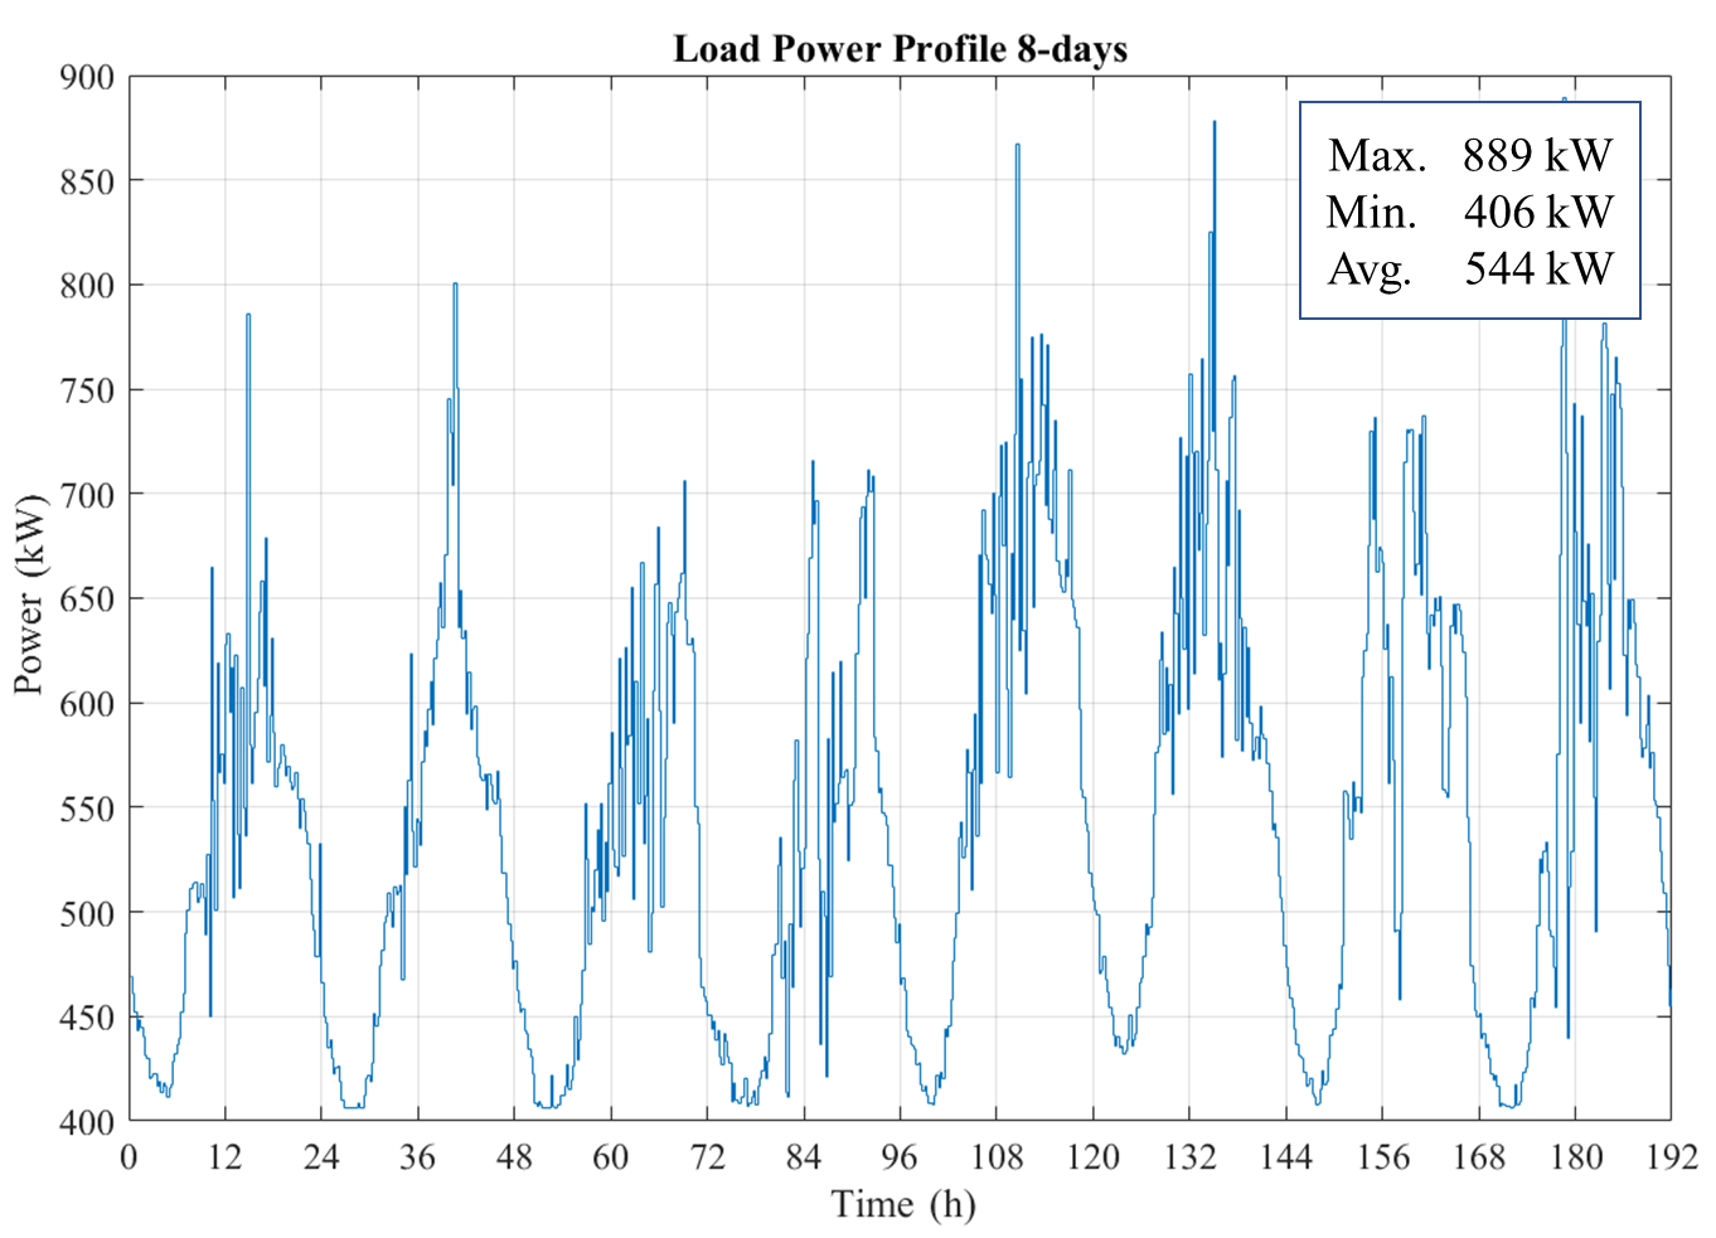
\includegraphics[width = 0.6\linewidth]{figs/A8/loadprofile.png}
    \caption{Eight day load profile}
    \label{fig:LOAD_PROFILE_8}
\end{figure}

\begin{figure}[!ht]
    \centering
    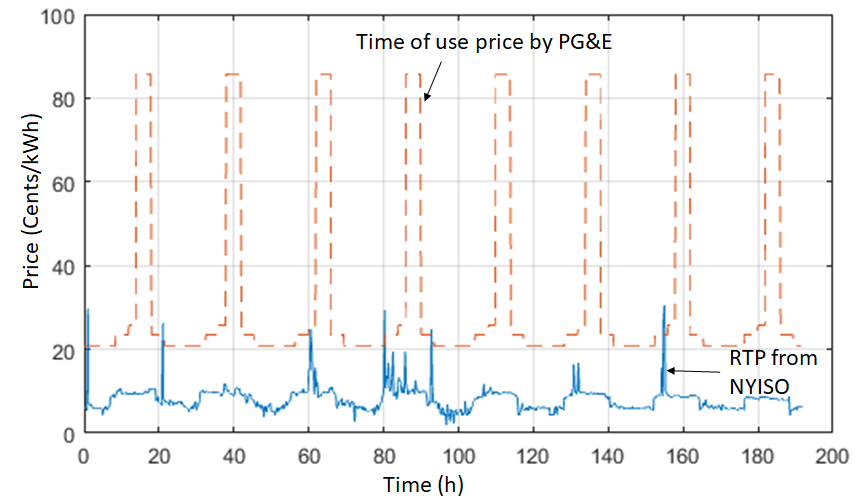
\includegraphics[width = 0.5\linewidth]{figs/A8/Price_profiles.png}
    \caption{Eight day RTP profile NYISO}
    \label{fig:RTP_PROFILE_8}
\end{figure}

% \begin{figure}[!ht]
%     \centering
%     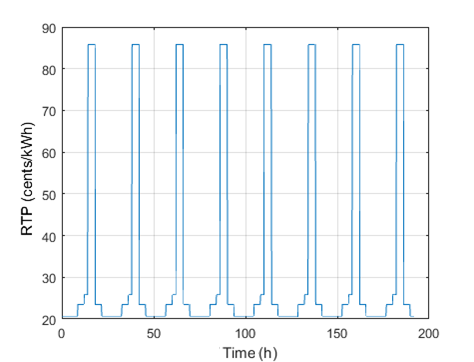
\includegraphics[width = \linewidth]{figs/PGNE_PRICE.png}
%     \caption{Eight day RTP profile PG\&E}
%     \label{fig:PGNE_PRICE}
% \end{figure}


\begin{figure}[!ht]
    \centering
    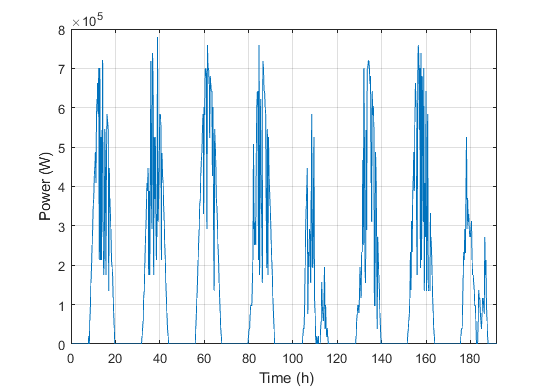
\includegraphics[width = 0.6\linewidth]{figs/A8/PV_PROFILE.png}
    \caption{Eight day PV profile}
    \label{fig:PV_PROFILE_8}
\end{figure}


